%!TEX root=paper.tex

\newpage
\section{Testing With High School Students}
\label{sec:demographics}

We tested our system with \stcnt students from a public highschool in Netherlands, representing three classes that have the same French teacher and are bilingual in Dutch and English. 

% \begin{added}
{\bf Usage Scenario. }
	The teacher asked the students to use the system for {\bf supplementary reading}. 
	% , aside from the other activities that were done in the class. 
	He encouraged them to read texts they found interesting and to build up their own {\em personalized portfolio of words}, complementary to the list of mandatory words that were common in every class.
	
	For every half an hour of usage, the students had to write a brief report on how they spent their time and submit it to the teacher. The teacher could then decide to selectively test them on the basis of their reports. 
	% This was a requirement from the teacher and based on a strategy 
	The teacher had used this strategy in the past with other software that he used in class. 
	% This might have affected negatively the willingness of the students to spend time on the platform.
% \end{added}


{\bf Deployment.} At the beginning of June 2017 we introduced the system and its usage to each of the three classes. With few exceptions the students created an account and started using the system the latest on June 9th and until the end of the month, which coincided with the end of the study year. 
% \begin{added}
Students used personal computers and Android/iOS devices.
% \end{added}

Before creating accounts on our platform, we asked the participants to answer a survey about their current level of knowledge, learning strategies, and reading interests. A handful of the participants, who were not in class when we presented the system, did not fill the survey.

When asked whether they have favorite topics they would like to read about, half of the students mentioned various topics while the other half did not answer the question. From the topics that they mentioned as possible interests some of the more popular were: sports, music, travel, lifestyle, fashion, movies, and somebody mentioned as interest {\em ``no politics''}.


In collaboration with the teacher we seeded the system with a variety of French news and blogs that cover the aforementioned aspects: 1Jour1Actu, L'Equipe, La Blogoteque, Le Figaro, Le Monde. 
% 
% \begin{added}
	% 
	Even if the source of readings was not actually the entire web, practically, having many dozens of news articles daily (only Le Figaro has usually more than forty in a day) offers sufficient opportunity for the free choice of individually interesting articles. 
	% {\em reading personalization} 
	% We could have added even 
	
% \end{added}



We deployed the system with the translations to English since, based on our experience translation APIs are of higher quality when one of the languages is English and because the students and their teacher were comfortable with the idea.\footnote{We made it clear to the students that they can ask us, and we will modify their personal account in such a way as to receive translations in Dutch. None of the students requested this.}

We also invited the students to send us feedback at any time if they encounter problems or if they have ideas for improvement. Several of them did email. Towards the end of the month, we deployed several in-app focused pop-up questions using a customer opinion elicitation service called HotJar. After the month was over we sent out a follow-up questionnaire.


% \subsection{The Teacher Dashboard}

We also provided the teacher with a dashboard to see the activity of the students: the texts that were read and translations they requested. This chronological activity view is available also for the student who can solely see their own history.


% \begin{figure}[h!]
% \centering
%   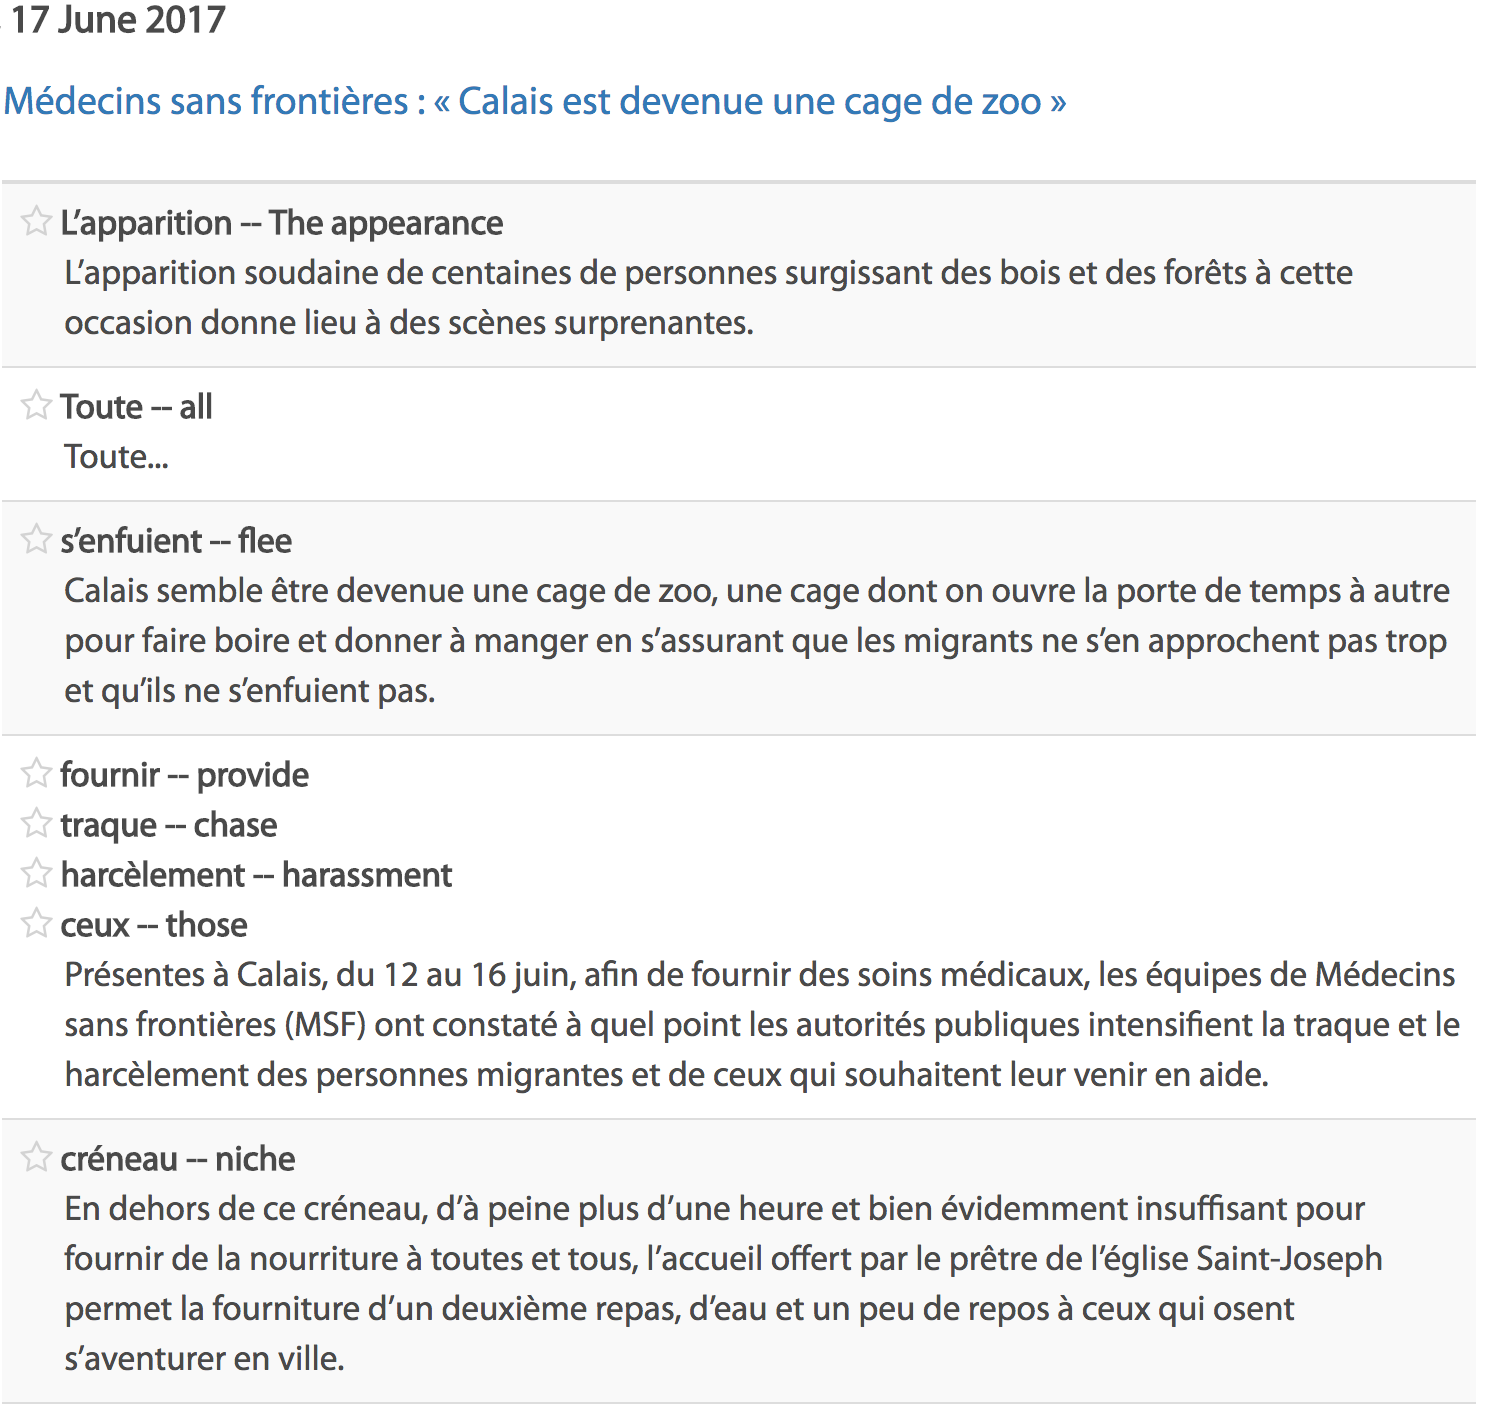
\includegraphics[width=0.8\columnwidth]{figures/teacher_dashboard.png}
%   \caption{A teacher can see the log of the words that a student looked up, their chosen translations, and the corresponding contexts}{
%   \label{fig:teacher}
%   }
% \end{figure}





{\bf Demographics.} 
The participants that filled the survey were 54 female and 15 male with ages below 18. Based on their self characterization, 53 students are level B1 (i.e. can understand the main points of clear standard speech, can narrate an event, experience or dream) and 16 are level A2 (i.e. can describe their surroundings and communicate immediate needs). 














% To talk to Nienke about the other types of analysis we can do on this data